\documentclass{article}
\usepackage[utf8]{inputenc}
\usepackage[T1]{fontenc}
\usepackage{xcolor}
\usepackage{tikz}
\usepackage{pgfplots}
\usepackage{tikz}
\usepackage{amsmath}
\usepackage{tikz}
\usetikzlibrary{calc}
\usetikzlibrary{positioning, shapes}

\begin{document}

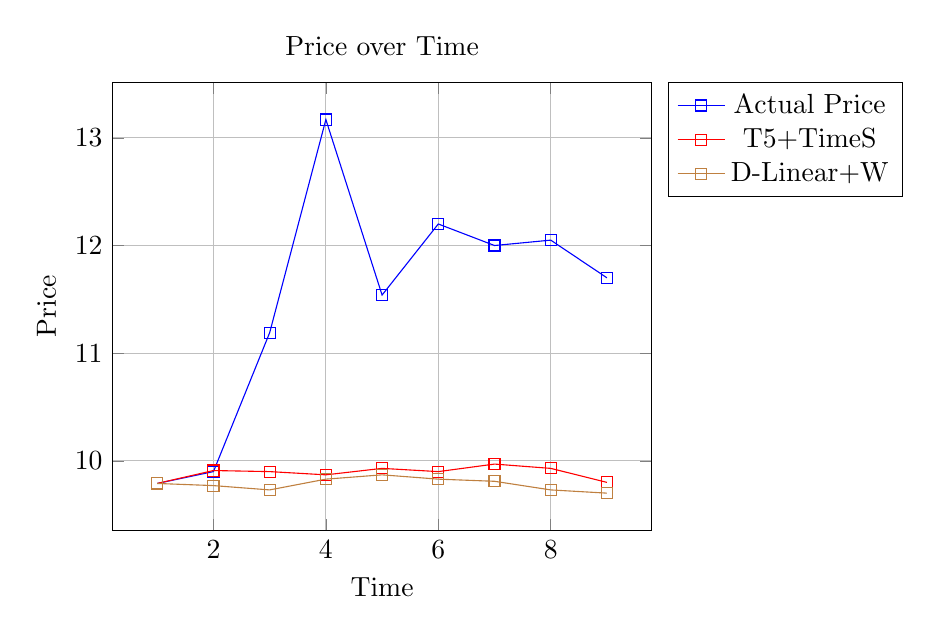
\begin{tikzpicture}
    \begin{axis}[
        title={Price over Time},
        xlabel={Time},
        ylabel={Price},
        grid=major,
        legend entries={Actual Price,T5+TimeS,D-Linear+W},
        legend pos=outer north east
    ]
    \addplot[
        color=blue,
        mark=square,
    ] coordinates {
        (1,9.7900	)
        (2, 9.9000)
        (3,11.1900)
        (4, 13.1700)
        (5, 11.5400)
        (6,12.2000)
        (7, 12.0000)
        (8, 12.0500)
        (9, 11.7000	)
    };
    \addplot[
        color=red,
        mark=square,
    ] coordinates {
        (1,9.79)
        (2, 9.91)
        (3,9.90)
        (4, 9.87)
        (5, 9.93)
        (6,9.90)
        (7, 9.97)
        (8, 9.93)
        (9, 9.80)
    };
     \addplot[
        color=brown,
        mark=square,
    ] coordinates {
         (1,9.79)
         (2, 9.77)
        (3,9.73)
        (4, 9.83)
        (5, 9.87)
        (6,9.83)
        (7, 9.81)
        (8, 9.73)
        (9, 9.70)
    };
    \end{axis}
\end{tikzpicture}

\end{document}